\chapter{Ứng dụng ngôn ngữ Rust}
\section{Chọn vi xử lý để thực hiện lập trình nhúng trong Rust}
Trước khi thực hiện lập trình nhúng cho bất kỳ hệ thống nào, ta phải chọn một vi điều khiển phù hợp cho hệ thống đó trước.

Trước hết, tôi đưa ra một số vi xử lý thông dụng, phù hợp, được sử dụng để giảng dạy về lập trình hệ nhúng ở trường Đại học Bách Khoa TP.HCM, so sánh chúng và từ đó chọn một vi xử lý phù hợp với nhu cầu.
\subsection{Một số vi xử lý thông dụng}
\subsubsection{MSP-EXP430G2 Evaluation board}
\begin{figure}[ht]
\centering
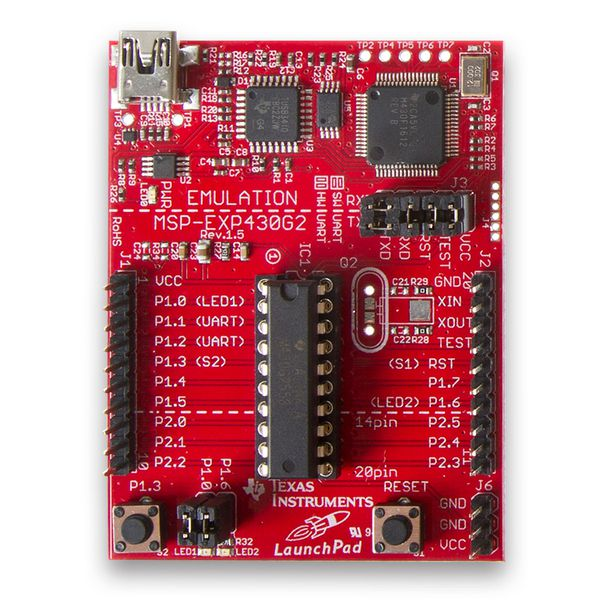
\includegraphics[scale=0.35]{images/launchpad-mspexp430g2-02.jpg}
\caption{MSP-EXP430G2}
\end{figure}
\clearpage

MSP-EXP430G2 \cite{msp430_datasheet} (hay MSP430) là dòng vi điều khiển của Texas Instrument (TI), 16 bit, kiến trúc RISC được thiết kế đặc biệt cho siêu năng lượng thấp.

\textbf{Một số hiệu năng nổi bật của MSP430}
\begin{itemize}
    \item CPU 16 bit tốc độ \si{16\MHz}.
    \item 16 KB Flash.
    \item 512B SRAM.
\end{itemize}

\textbf{Ưu điểm}: Giá thành rẻ, nhỏ gọn, đầy đủ các ngoại vi thông dụng. Có bộ thư viện phong phú dễ dàng thực hiện lập trình nhúng trên nhiều lĩnh vực.

\textbf{Nhược điểm}: Khá ít bộ nhớ SRAM, cũng như tốc độ CPU còn hạn chế, và CPU chỉ hỗ trợ tính toán 16 bit nên sẽ khó có thể thực hiện tính toán nặng trên MSP430.

\subsubsection{STM32F103C8T6 - Blue Pill}
\begin{figure}[ht]
\centering
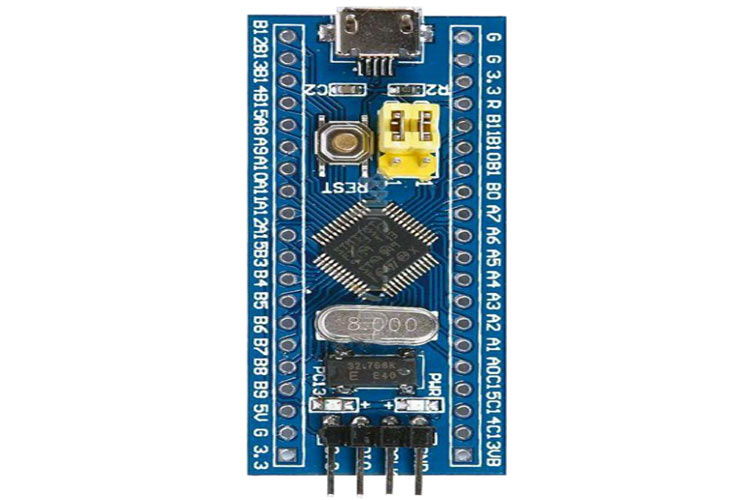
\includegraphics[scale=0.35]{images/STM32-Blue-Pill-Development-Board.jpg}
\caption{STM32 Blue Pill}
\end{figure}
STM32F103C8T6 \cite{blue_pill_datasheet} (hay Blue Pill) là một vi xử lý rất thông dụng của ST-Microelectronics, sử dụng CPU Arm-Cortex M3, 32 bit với giá thành rẻ.

\textbf{Một số hiệu năng nổi bật của Blue Pill}
\begin{itemize}
    \item CPU ARM-Cortex M3 32 bit tốc độ \si{72\MHz}, 1.25 DMIPS/MHz.
    \item 128 KB Flash.
    \item 20 KB SRAM.
\end{itemize}

\textbf{Ưu điểm}: Giá thành rẻ, nhỏ gọn, đầy đủ các ngoại vi thông dụng. CPU mạnh mẽ. Kèm theo một số ngoại vi khác như RTC.

\textbf{Nhược điểm}: Vì Blue Pill sử dụng CPU ARM-Cortex M3 nên một số tính năng tính toán nặng như DSP sẽ không được phần cứng hỗ trợ. Ngoài ra, ta không thể flash trực tiếp chương trình lên Blue Pill được mà phải thông qua một Bootloader như ST-Link/V2 \cite{stlinkv2_datasheet}.

\subsubsection{Arduino Uno R3}
\begin{figure}[ht]
\centering
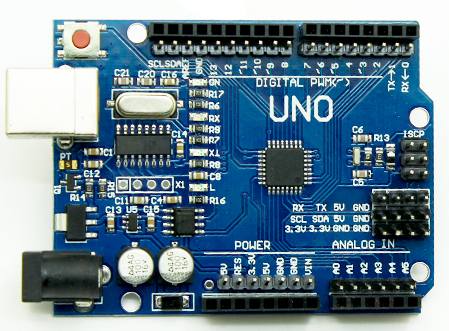
\includegraphics[scale=0.75]{images/Arduino-Uno-R3-SMD.jpg}
\caption{Arduino Uno R3}
\end{figure}

Arduino Uno R3 \cite{arduino_datasheet} là loại phổ biến và dễ sử dụng nhất trong các dòng Arduino hiện nay cũng như tương thích với nhiều Arduino Shield.

\textbf{Một số hiệu năng nổi bật của Arduino Uno R3}
\begin{itemize}
    \item CPU ATmega328P 8 bit tốc độ \si{16\MHz}.
    \item 32 KB Flash.
    \item 1 KB EEPROM.
    \item 2 KB SRAM.
\end{itemize}

\textbf{Ưu điểm}: Giá thành rẻ, nhỏ gọn, đầy đủ các ngoại vi thông dụng.

Có rất nhiều thư viện abstraction C/C++ chất lượng cao, dễ sử dụng.

\textbf{Nhược điểm}: Hiệu năng tính toán của Arduino Uno R3 tương đối hạn chế.

AVR \mintinline{bash}{avr-unknown-gnu-atmega328} là đối tượng bậc 3 của bộ compiler trong Rust \cite{rustc_book}, vì vậy lập trình trên vi điều khiển này sẽ gặp nhiều chướng ngại vật, khó có thể đánh giá khách quan về hệ thống.

\clearpage
\subsubsection{EK-TM4C123G}
\begin{figure}[ht]
\centering
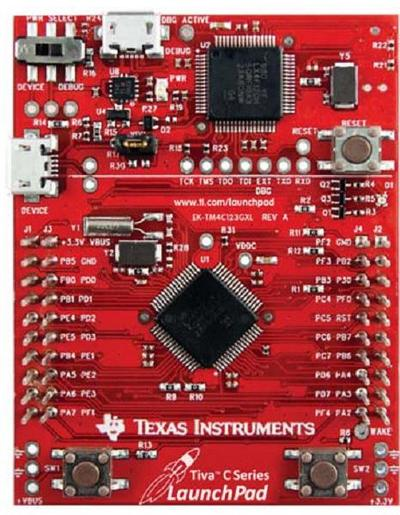
\includegraphics[scale=0.5]{images/kit_tivac.jpg}
\caption{Evaluation Kit EK-TM4C123G}
\end{figure}

EK-TM4C123G \cite{tivac_datasheet} (hay kit Tiva C launchpad) được phát triển bởi tập đoàn Texas Instruments để thay thế cho sản phẩm Stellaris Launchpad đã dừng sản xuất trước đó.
Dòng Tiva C 32-bit được sử dụng trong đề tài này có một thiết kế hiện đại cùng tập lệnh phong phú và hệ sinh thái về code nhúng giàu có
đã đẩy nhanh việc giảng dạy về lập trình nhúng nói chung trong môi trường trường học cũng như cũng đủ mạnh mẽ để có thể phát triển thêm lên để sử dụng trong môi trường công nghiệp hiện đại.

\textbf{Một số hiệu năng nổi bật của Tiva C launchpad}
\begin{itemize}
    \item CPU ARM-Cortex M4F 32 bit tốc độ \si{80\MHz}, 1.25 DMIPS/MHz.
    \item 256 KB Flash.
    \item 32 KB SRAM.
    \item 2 KB EEPROM.
\end{itemize}

\textbf{Ưu điểm}: Giá thành rẻ, nhỏ gọn, mạnh mẽ. Có bộ thư viện phong phú dễ dàng thực hiện lập trình nhúng trên nhiều lĩnh vực.
Khả năng hoạt động với chế độ tiết kiệm điện để hoạt động liên tục, phù hợp cho việc áp dụng cho môi trường thực tiễn.

\textbf{Nhược điểm}: Giá thành vẫn còn đắt hơn so với một số thiết bị STM32 với cùng hiệu năng. (khoảng 350000 VNĐ ở thời điểm tháng 06/2021)

\clearpage
\subsubsection{STM32F411 Discovery}
\begin{figure}[ht]
\centering
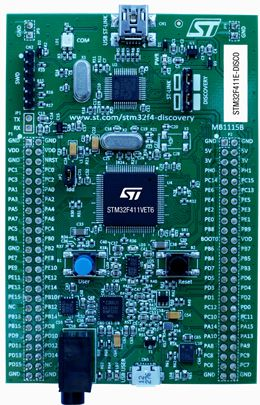
\includegraphics[scale=0.5]{images/en-stm32f411e-disco.jpg}
\caption{STM32F411 Discovery}
\end{figure}

STM32F411 \cite{discovery_datasheet} (hay STM32 Discovery) là một phiên bản nâng cấp của kit STM32F407 Discovery được sử dụng rất phổ biển hiện nay trong các nghiên cứu về dòng ARM STM32F4.
Kit có tích hợp sẵn mạch nạp ST-Link/V2, các ngoại vi như cảm biến gia tốc, từ trường, audio, v.v..

\textbf{Một số hiệu năng nổi bật của STM32 Discovery}
\begin{itemize}
    \item CPU ARM-Cortex M4 + DSP Core 32 bit tốc độ \si{100\MHz}, 1.25 DMIPS/MHz.
    \item 512 KB Flash.
    \item 128 KB SRAM.
\end{itemize}

\textbf{Ưu điểm}: Các thông số hiệu năng cực kỳ mạnh mẽ, kèm theo DSP Core cũng như tích hợp một số ngoại vi khác như cảm biến gia tốc, từ trường, audio, v.v..

\textbf{Nhược điểm}: Giá thành tương đối đắt (khoảng 500.000 VNĐ ở thời điểm tháng 06/2021).

\subsubsection{Raspberry Pi 3 Model B+}
\begin{figure}[ht]
\centering
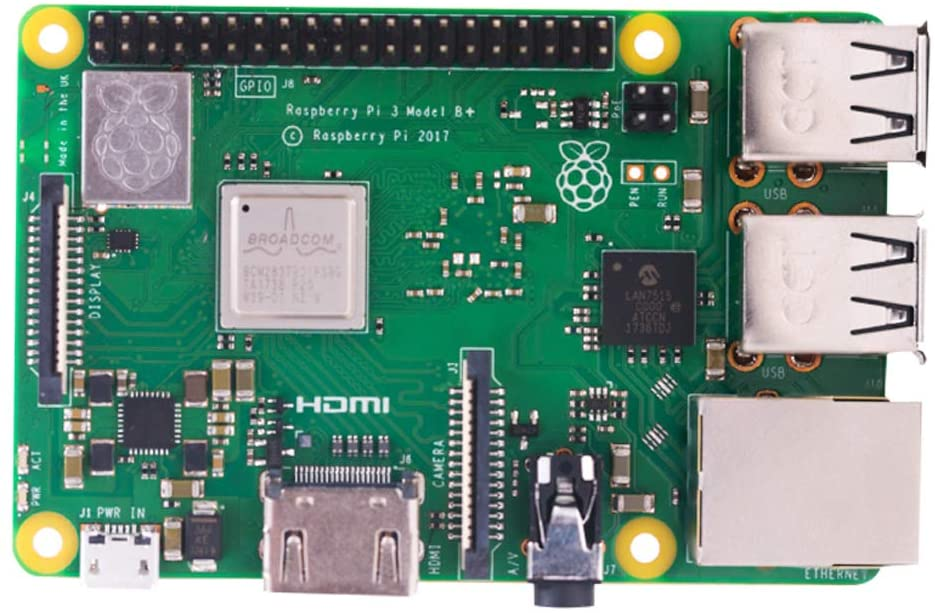
\includegraphics[scale=0.25]{images/raspberry-pi-model-3bplus.jpg}
\caption{Raspberry Pi 3 Model B+}
\end{figure}
Máy tính Raspberry Pi 3 Model B+ \cite{raspberry_datasheet} là một trong những sản phẩm tương đối mới, nổi bật với 4 nhân 64 bit CPU ARM-Cortexv8 với tốc độ lên đến 1.4 GHz.
Máy tính Raspberry Pi 3 Model B+ đủ mạnh để có thể chạy được một hệ điều hành như Linux.

\textbf{Một số hiệu năng nổi bật của Raspberry Pi 3 Model B+}
\begin{itemize}
    \item Quad-core CPU ARM-Cortex-A53 64 bit tốc độ \si{1.2\GHz}.
    \item 1 GB RAM.
    \item Đi kèm với VideoCore IV multimedia/3D graphic core.
\end{itemize}

\pagebreak
\textbf{Ưu điểm}: Có hiệu năng vượt trội hơn hẳn tất cả các vi điều khiển đã liệt kê trước.

Thư viện hỗ trợ cho Raspberry Pi có thể được xem là một trong những thư viện đầy đủ nhất.

Raspberry Pi 3 Model B+ đủ mạnh để có thể chạy hệ điều hành Linux nên ta có thể lập trình nhúng cực kỳ dễ dàng và hiệu quả.

\textbf{Nhược điểm}: Giá thành đắt. Tại thời điểm tháng 06/2021 thì giá thành của một kit Raspbery Pi 3 Model B+ là khoảng 1100000 VNĐ chưa kèm phụ kiện.

\subsection{Lựa chọn vi điều khiển}

Ở đây, để thực hiện ứng dụng Rust cho một hệ thống nhúng thực tế, tôi đưa ra một số yêu cầu để thử nghiệm ngôn ngữ này.

\begin{itemize}
    \item Vi điều khiển này có đầy đủ các chức năng của một vi điều khiển thông dụng, để ta có thể dễ dàng thử nghiệm toàn bộ những ngoại vi cơ bản.
    \item Vi điều khiển này được hỗ trợ tương đối tốt, cả trong C lẫn Rust để ta có thể dễ dàng so sánh kết quả trong quá trình thiết kế hệ thống nhúng.
    \item Vì Rust là một ngôn ngữ cấp thấp, tôi muốn thử nghiệm tính toán nặng trên vi điều khiển để kiểm tra về tốc độ của Rust trong một hệ thống thực tế.
    \item Giá thành tương đối rẻ.
        Trong lập trình nhúng, thiết kế các hệ thống với những giới hạn nhất định về phần cứng cũng như về giá thành của hệ thống là một công việc mà người thiết kế hệ thống thường xuyên gặp phải.
        Vì vậy, Rust phải hỗ trợ những vi điều khiển giá rẻ, không được giới hạn bởi các vi điều khiển cao cấp.
\end{itemize}

Dựa trên các yêu cầu này, có thể thấy có hai lựa chọn về vi xử lý để thực hiện những yêu cầu này là kit Tiva C và kit STM32 Discovery.

Ở đây, tôi quyết định chọn kit Tiva C làm đối tượng để nghiên cứu trong đề tài này vì giá thành của nó rẻ hơn so với kit STM32 Discovery.

\section{Viết phần mềm nhúng cho vi điều khiển trong Rust}
Trước khi thực hiện viết chương trình nhúng cho vi điều khiển, ta cần chuẩn bị một số công cụ để thực hiện điều này.

\begin{itemize}
    \item Các công cụ của Rust: chi tiết cài đặt có thể xem tại website chính thức Rust Programming Language \cite{rust_website}.
    \item Cargo clone: cài đặt thông qua \mintinline{bash}{cargo install cargo-clone} \cite{cargo_clone}.
    \item Một số các công cụ biên dịch mã cho đối tượng ARM:

    \mintinline{bash}{arm-none-eabi-gcc arm-none-eabi-ar arm-none-eabi-objcopy}
    \item Công cụ flash cho Tiva C: \mintinline{bash}{lm4flash} \cite{lm4tools}.
    \item GDB cho đối tượng ARM: \mintinline{bash}{gdb-arm-none-eabi} \cite{gdb_website}.
    \item OpenOCD: \mintinline{bash}{openocd} \cite{openocd_website}.
\end{itemize}

Ở đây, vì kit Tiva C có một BSP là \mintinline{bash}{stellaris-launchpad} \cite{stellaris_launchpad_bsp} nên tôi sẽ sử dụng crate này để đấy nhanh tiến độ thực hiện lập trình. \label{lbl:tivac_bsp}

Trước hết, ta tham khảo cấu trúc của crate \mintinline{bash}{stellaris-launchpad} qua ví dụ \ref{lst:stellaris_launchpad_structure}.

\begin{listing}
\dirtree{%
.1 stellaris-launchpad/.
.2 .cargo.
.2 examples.
.2 src.
.2 .gdbinit.
.2 Cargo.lock.
.2 Cargo.toml.
.2 build.rs.
.2 memory.x.in.
}
\caption{Cấu trúc của crate BSP stellaris-launchpad}
\label{lst:stellaris_launchpad_structure}
\end{listing}

Ta thấy nó tương tự với cấu trúc một dự án Rust cơ bản (xem trang \pageref{lbl:basic_rust_proj_structure}), nhưng có thêm một số file khác.
Tôi đi tiến hành phân tích về công dụng của các file này.

\textbf{.gdbinit}

File này chứa các lệnh của GDB sẽ thực hiện khi khởi động GDB \cite{gdbinit}.

\textbf{build.rs}

Một số thư viện cần phải biên dịch thêm một số mã nguồn khác (như C), một số khác cần phải link với các thư viện C trên hệ thống hay biên dịch từ mã nguồn.

Vì \mintinline{bash}{cargo} không thể thực hiện những điều này nên file \mintinline{bash}{build.rs} được sử dụng để thông báo cho \mintinline{bash}{cargo} rằng nó sẽ không thực hiện biên dịch mã trực tiếp mà sẽ thông qua một số bước khác được định nghĩa trong file này \cite{cargo_book}.

\textbf{memory.x}

File này chứa thông số về địa chỉ FLASH và địa chỉ RAM cũng như độ lớn của chúng.

Ví dụ \ref{lst:memory_x} là nội dung file \mintinline{bash}{memory.x} của crate BSP \mintinline{bash}{stellaris-launchpad}.

\begin{listing}[ht]
\begin{plaintext}
MEMORY
{
    FLASH (rx) : ORIGIN = 0x00000000, LENGTH = 0x00040000
    RAM (rwx) : ORIGIN = 0x20000000, LENGTH = 0x00008000
}
\end{plaintext}
\caption{Một ví dụ về file memory.x}
\label{lst:memory_x}
\end{listing}

Dựa theo hướng dẫn của crate, ta thấy rằng, các dự án sẽ được viết và đặt trong thư mục \mintinline{bash}{examples}.

Biên dịch sử dụng lệnh \mintinline{bash}{cargo build --example <name> --release}.

Chuyển thành dạng binary sử dụng lệnh \mintinline{bash}{arm-none-eabi-objcopy -O binary tgt dst}

Và cuối cùng là flash file binary lên kit bằng lệnh \mintinline{bash}{lm4flash dst.bin}

Tôi tiến hành viết một số chương trình có độ khó từ đơn giản đến phức tạp để thử nghiệm Rust trên Tiva C.

\subsection{Chương trình nháy LED}\label{lbl:rust_blinky}
Chương trình nháy LED được xem là chương trình đơn giản nhất trong một hệ thống nhúng.
Tôi tiến hành thực hiện viết một chương trình nháy LED để làm quen với cách làm việc với một đề tài hệ thống nhúng trong Rust.

Để thực hiện một chương trình nháy LED, tôi trước tin thực hiện trực tiếp thông qua HAL của kit Tiva C \cite{tm4c_hal}.
Chương trình có nội dung như trong ví dụ \ref{code:tivac_hal_blinky} sau.

\begin{listing}[ht]
\begin{rustcode}
#![no_std]
#![no_main]

use panic_halt as _;

use cortex_m_rt::entry;
use tm4c123x_hal::{self as hal, prelude::*};

#[entry]
fn main() -> ! {
    let p = hal::Peripherals::take().unwrap();

    let mut sc = p.SYSCTL.constrain();
    sc.clock_setup.oscillator = hal::sysctl::Oscillator::Main(
        hal::sysctl::CrystalFrequency::_16mhz,
        hal::sysctl::SystemClock::UsePll(hal::sysctl::PllOutputFrequency::_80_00mhz),
    );
    let clocks = sc.clock_setup.freeze();

    let portf = p.GPIO_PORTF.split(&sc.power_control);
    let mut led = portf.pf1.into_push_pull_output();

    let mut delay = hal::delay::Delay::new(core_peripherals.SYST, &clocks);

    loop {
        led.set_high();
        delay.delay_ms(500u32);
        led.set_low();
        delay.delay_ms(500u32);
    }
}
\end{rustcode}
\caption{Ví dụ blinky sử dụng Tiva C HAL}
\label{code:tivac_hal_blinky}
\end{listing}

Tôi phân tích một vài điểm chưa được giải thích ở trong các phần trước từ ví dụ này.

\begin{itemize}
    \item Đầu tiên là hai thuộc tính \mintinline{rust}{#[no_std]} và \mintinline{rust}{#[no_main]} được đặt ở đầu chương trình.

        \mintinline{rust}{#[no_std]} như đã phân tích ở phần \ref{lbl:no_std_crates} (trang \pageref{lbl:no_std_crates}), ở đây được đặt ra để báo với compiler là chương trình này không sử dụng thư viện std.

    \mintinline{rust}{#[no_main]} thông báo với compiler rằng chương trình này sẽ không sử dụng symbol \mintinline{bash}{main} thông thường để làm entry point. Thông thường, một chương trình Rust suy đoán một số thông số từ môi trường mà chương trình sẽ chạy trên. Tuy nhiên ở trong môi trường nhúng, các thông số này có thể không đúng, vì vậy để chương trình được biên dịch chính xác ta cần phải có thuộc tính này \cite{rust_reference, embedonomicon}.

    \item \mintinline{rust}{use panic_halt as _;} đoạn mã này tạo một hàm \mintinline{bash}{panic} để khi chương trình gặp lỗi thì nó sẽ chuyển sang chạy một vòng lặp vô hạn trong hàm này.
    \item \mintinline{rust}{#[entry]} thông báo với compiler đây là điểm entry của chương trình.
        Thuộc tính này được lấy từ crate \mintinline{bash}{cortex-m-rt-macros} để từ đó kết hợp với file \mintinline{bash}{memory.x} để flash chương trình đúng vào địa chỉ dùng cho bộ nhớ FLASH \cite{cortex_m_rt}.
\end{itemize}

Từ trong chương trình main, các lệnh để thực hiện khởi động ngoại vi, thiết lập xung clock có thể thấy tương đối tương tự như ta sử dụng các hàm trong C để thực hiện các thao tác này, chỉ có một điểm ở đây cần chỉ ra đó là khi khởi động LED (pin PF1 trên kit), ta phải đặt biến này ở dạng mutable vì khi thực hiện nháy LED thì ta phải thay đổi trạng thái ON/OFF của LED, nếu không khởi động ở dang mutable thì chương trình khi biên dịch sẽ gặp lỗi. Điều này tương tự với biến delay.

Có thể thấy rằng, khi có HAL, thực hiện một chương trình đơn giản như nháy LED là tương đối đơn giản, dễ hiểu và nhanh chóng.
Giao diện này là ở mức khá cao, có thể nói là cao hơn so với thư viện HAL TivaWare \cite{tivac_tivaware}, khá tương đồng với cách sử dụng HAL như trong IDE của Arduino.

Tuy nhiên, ta vẫn có thể đi lên một nấc abstraction cao hơn nữa nhờ sử dụng BSP của kit Tiva C (đã giới thiệu ở trang \pageref{lbl:tivac_bsp}).
Ta thực hiện viết viết một file \mintinline{bash}{blinky.rs} với nội dung như trong ví dụ \ref{code:tivac_bsp_blinky}.

\begin{listing}[ht]
\begin{rustcode}
#![no_std]
#![no_main]

extern crate embedded_hal;
extern crate stellaris_launchpad;
extern crate tm4c123x_hal;

use embedded_hal::blocking::delay::DelayMs;
use embedded_hal::digital::v2::OutputPin;

#[no_mangle]
pub fn stellaris_main(mut board: stellaris_launchpad::board::Board) {
    let mut delay = tm4c123x_hal::delay::Delay::new(
        board.core_peripherals.SYST,
        stellaris_launchpad::board::clocks(),
    );

    loop {
        board.led_red.set_high().unwrap();
        delay.delay_ms(500u32);
        board.led_red.set_low().unwrap();
        delay.delay_ms(500u32);
    }
}
\end{rustcode}
\caption{Ví dụ blinky sử dụng Tiva C BSP}
\label{code:tivac_bsp_blinky}
\end{listing}

Ở đây, khi sử dụng BSP ta thấy việc nháy LED còn đơn giản hơn nữa vì BSP đã thực hiện các việc như khởi động kit, thiết lập clock, các ngoại vi cơ bản (như các LED trên kit) cho chúng ta và trả về một biến mutable là \mintinline{bash}{board} để ta mượn và sử dụng nó.

\subsection{Sử dụng một vài ngoại vi đơn giản}\label{lbl:rust_peripheral}
Sau khi đã nắm được cách viết một chương trình cơ bản, tôi tiếp tục thực hiện tương tác với một vài ngoại vi cơ bản của kit.
Ở ví dụ này, tôi chọn hai ngoại vi đó là UART và bộ Timer trên kit để tạo xung PWM điều khiển LED của kit.
Nội dung của chương trình người đọc có thể tham khảo ở phần phụ lục. % TODO

Một vài hình về kết quả thực hiện có thể xem ở các hình \ref{fig:cycle_kit}, \ref{fig:cycle_uart_out}, \ref{fig:cycle_uart_read}.

\begin{figure}[ht]
\centering
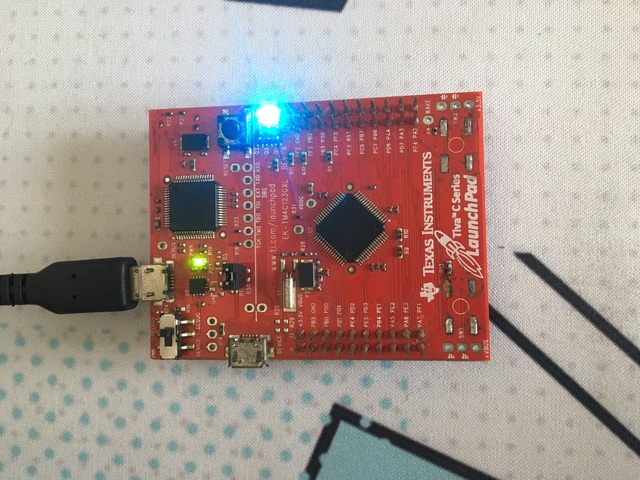
\includegraphics[scale=0.4]{images/cycle_kit.jpg}
\caption{LED cycle trên kit sử dụng Timer để tạo xung PWM}
\label{fig:cycle_kit}
\end{figure}

\begin{figure}[ht]
\centering
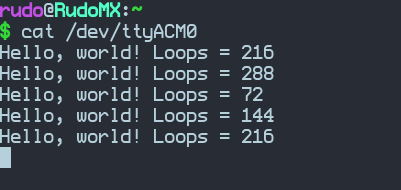
\includegraphics[scale=0.7]{images/cycle_uart_out.png}
\caption{Đọc thông tin từ kit sử dụng UART}
\label{fig:cycle_uart_out}
\end{figure}

\begin{figure}[ht]
\centering
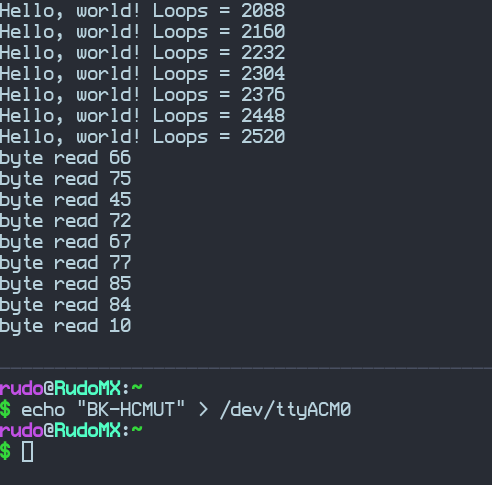
\includegraphics[scale=0.5]{images/cycle_uart_read.png}
\caption{Truyền thông tin cho kit sử dụng UART}
\label{fig:cycle_uart_read}
\end{figure}

\clearpage
\subsection{Tương tác với một vài thiết bị ngoài}\label{lbl:rust_mfrc522}
Sau khi đã làm quen với kit và các ngoại vi trên kit, bước tiếp theo tôi thực hiện tương tác với một số thiết bị ngoài.
Ở đây, tôi chọn 2 thiết bị là LCD 1602 \cite{lcd_datasheet} và module MFRC522 \cite{mfrc522_datasheet} thực hiện mô phỏng một hệ thống khóa cửa đơn giản.

Trước khi thực hiện hệ thống, tôi thực hiện gia công một mạch in đơn giản để thuận tiện hơn cho việc thực hiện hệ thống.
Schematic của hệ thống được trình bày ở hình \ref{fig:schematic}.
Kết quả thực hiện PCB và kết quả của hệ thống có thể xem ở các hình \ref{fig:pcb_routing}, \ref{fig:pcb_out}, \ref{fig:system}.

\begin{figure}[ht]
\centering
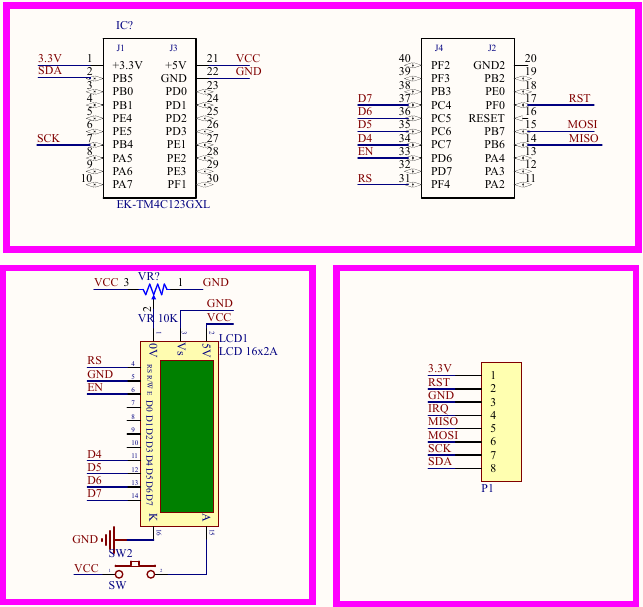
\includegraphics[scale=0.75]{images/schematic.png}
\caption{Schematic của hệ thống RFID}
\label{fig:schematic}
\end{figure}

\begin{figure}[ht]
\centering
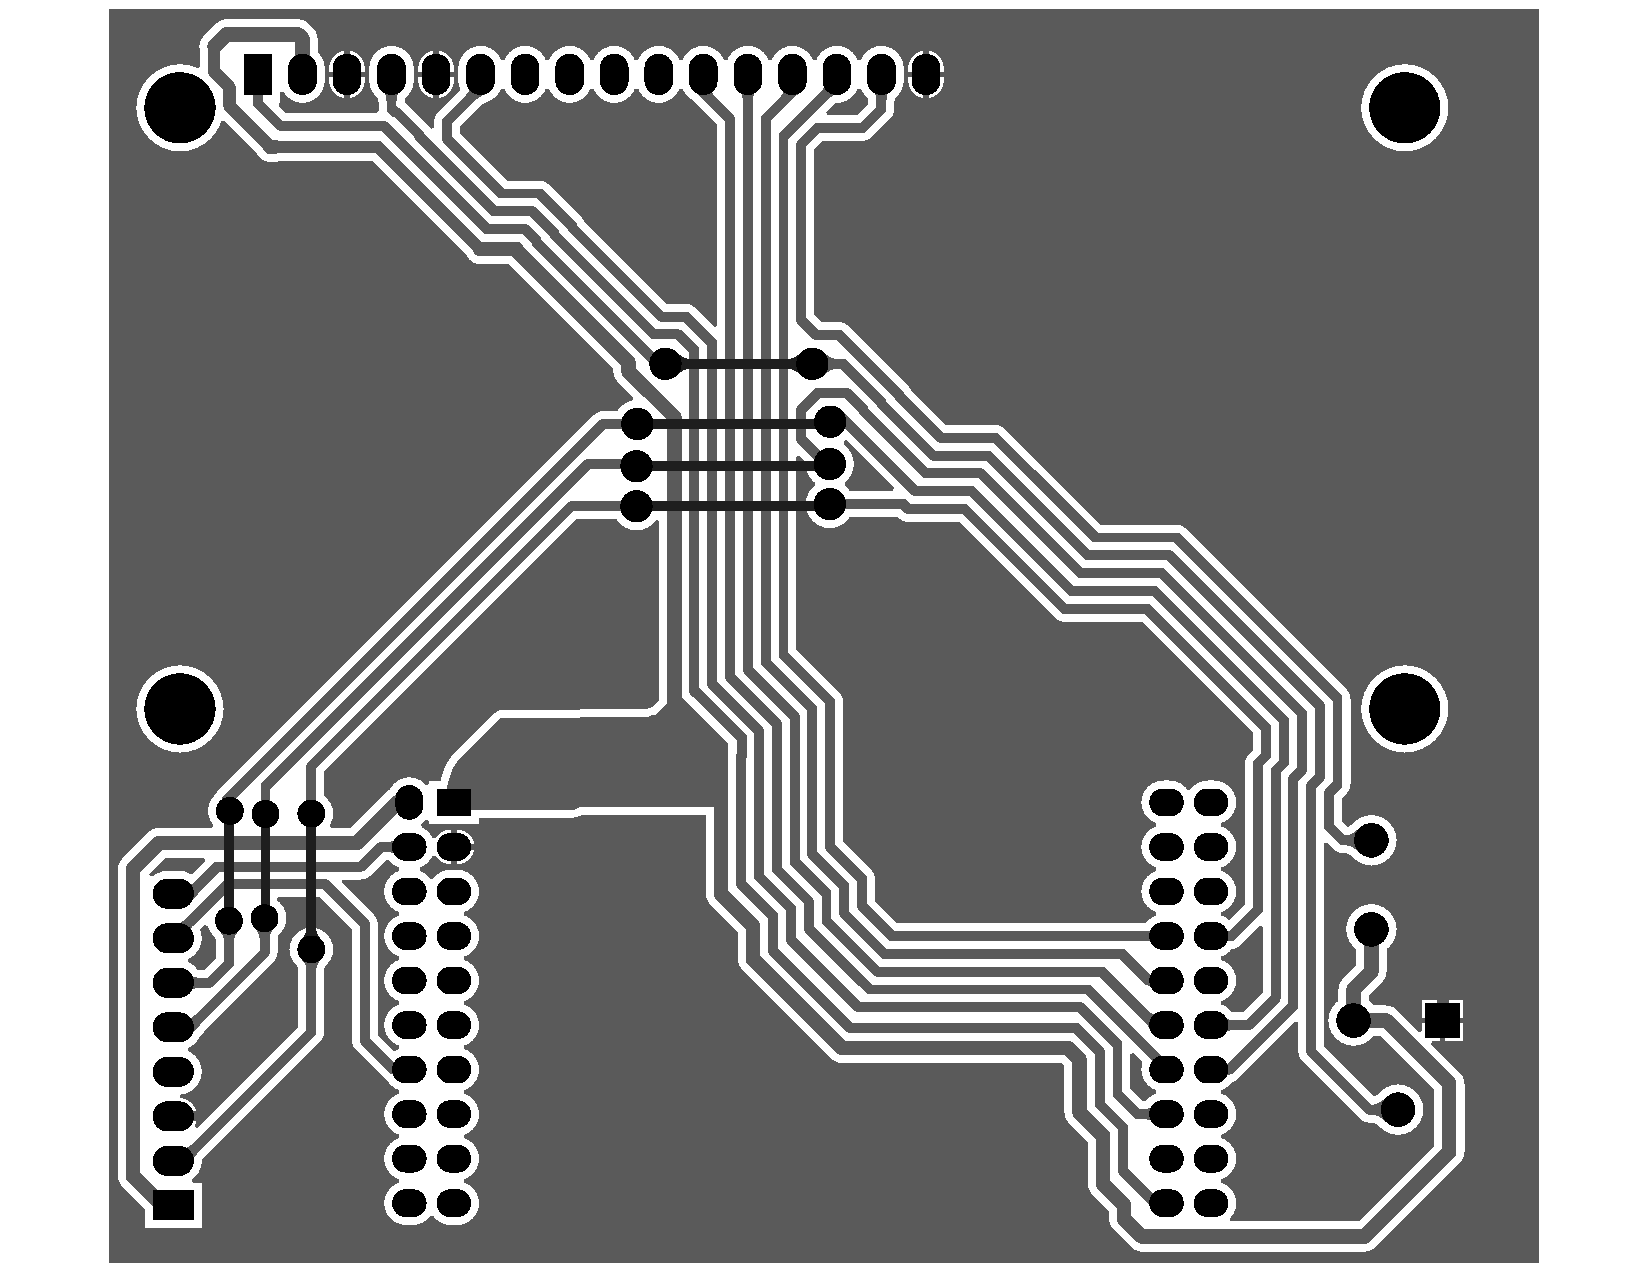
\includegraphics[scale=0.35]{images/routed.pdf}
\caption{Kết quả mạch sau khi thực hiện routing}
\label{fig:pcb_routing}
\end{figure}

\begin{figure}[ht]
\centering
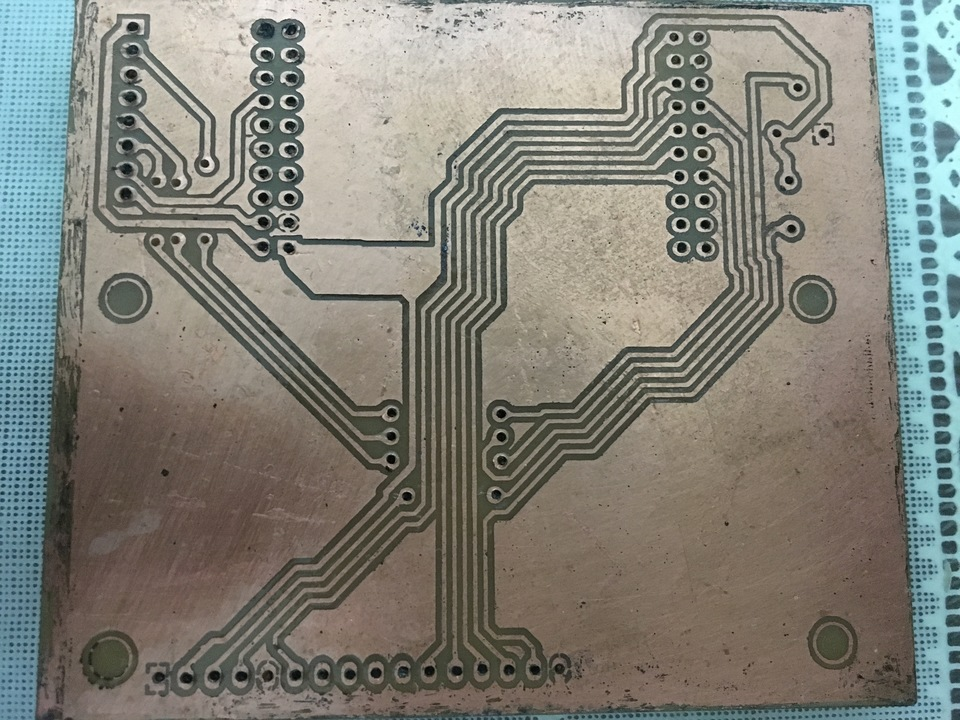
\includegraphics[scale=0.3]{images/board_output.jpg}
\caption{Kết quả mạch in}
\label{fig:pcb_out}
\end{figure}

\begin{figure}[ht]
\centering
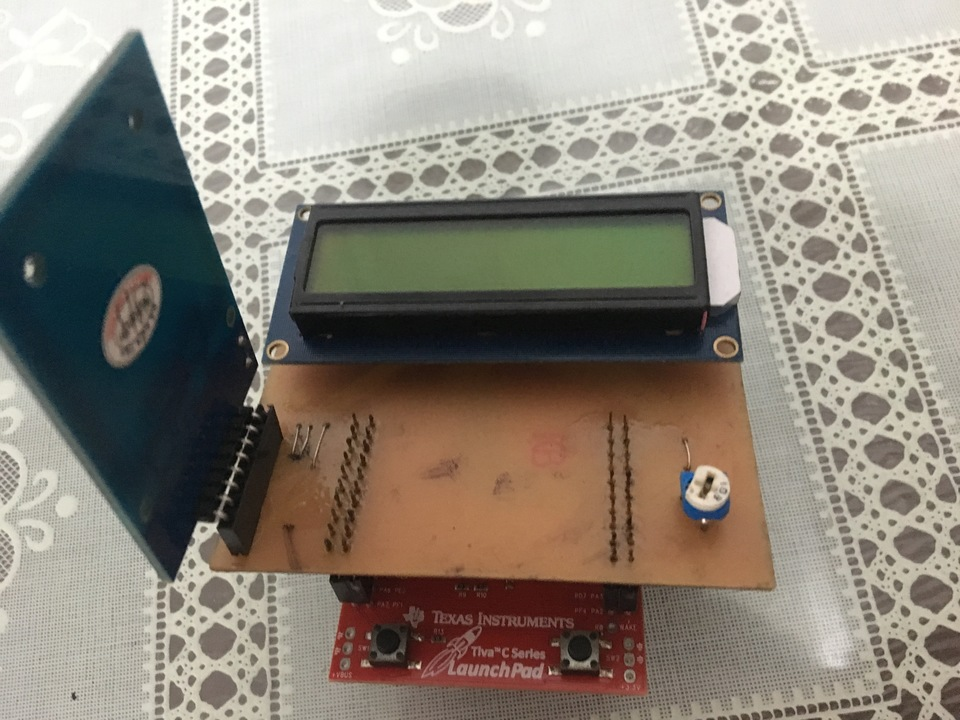
\includegraphics[scale=0.3]{images/board_finish.jpg}
\caption{Kết quả PCB đã gắn các linh kiện}
\label{fig:system}
\end{figure}

Lưu đồ giải thuật của chương trình được trình bày ở hình \ref{fig:rc522_flow}.

\begin{figure}[ht]
\centering
\begin{tikzpicture}[scale=0.75, every node/.style={scale=0.75}]
\tikzset{startstop/.style = {draw, rectangle, rounded corners, align=center, minimum width=3cm, minimum height=1cm}, >= latex,}
\tikzset{process/.style = {draw, rectangle, align=center, minimum width=3cm, minimum height=1cm}, >= latex,}
\tikzset{decision/.style = {draw, diamond, align=center, minimum width=3cm, minimum height=1cm}, >= latex,}
% Main nodes
\node (start) [startstop] {Bắt đầu};
\node (init) [process] [below=1cm of start] {Initialize hệ thống \\ Chọn chip slave};
\node (lcd_default) [process] [below=1cm of init] {Hiển thị dòng chữ \\ "Scan your card" ra LCD};
\node (card_check) [decision] [below=1cm of lcd_default] {Kiểm tra \\ có thẻ \\ được quét \\ không?};
\node (data_process) [process] [below=1cm of card_check] {Xử lý dữ liệu \\ đọc từ thẻ};
\node (led_blink) [process] [below=1cm of data_process] {Chớp LED trên board \\ báo hiệu đã đọc thẻ};
% Various coordinates
\coordinate[left=2cm of led_blink] (left_out);
\coordinate[above=0.5cm of card_check] (loop);
\coordinate[right=1cm of card_check] (right_card);
\coordinate[right=1cm of loop] (right_loop);
% Connectors
\draw [->] (start) -- (init);
\draw [->] (init) -- (lcd_default);
\draw [->] (lcd_default) -- (card_check);
\draw [->] (card_check) -- node [left] {Y} (data_process);
\draw [->] (card_check) -- node [above] {N} (right_card) |- (right_loop) |- (loop);
\draw [->] (data_process) -- (led_blink);
\draw [->] (led_blink) -- (left_out) |- (lcd_default);
\end{tikzpicture}
\caption{Lưu đồ giải thuật của hệ thống RFID}
\label{fig:rc522_flow}
\end{figure}

Nội dung của chương trình người đọc có thể tham khảo ở phần phụ lục. % TODO

Một vài hình về kết quả thực hiện có thể xem ở các hình \ref{fig:rc522_default}, \ref{fig:rc522_tag}, \ref{fig:rc522_card}, \ref{fig:rc522_student}.

\begin{figure}[ht]
\centering
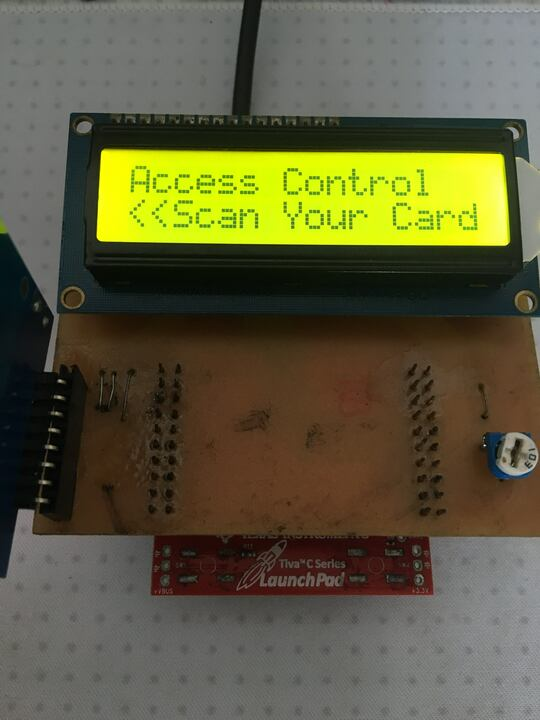
\includegraphics[scale=0.3]{images/mfrc522_default.jpg}
\caption{Kết quả hệ thống MFRC522 - Hệ thống ở trạng thái mặc định}
\label{fig:rc522_default}
\end{figure}

\begin{figure}[ht]
\centering
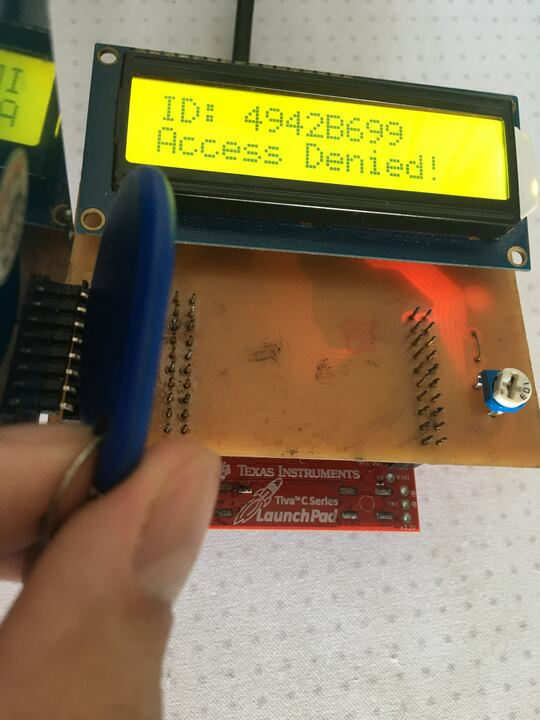
\includegraphics[scale=0.3]{images/mfrc522_tag.jpg}
\caption{Kết quả hệ thống MFRC522 - Sử dụng tag đi kèm}
\label{fig:rc522_tag}
\end{figure}

\begin{figure}[ht]
\centering
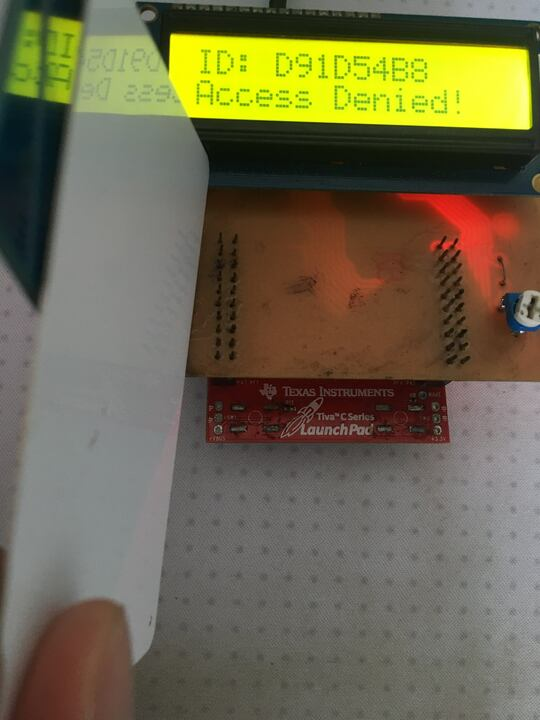
\includegraphics[scale=0.3]{images/mfrc522_card.jpg}
\caption{Kết quả hệ thống MFRC522 - Sử dụng card đi kèm}
\label{fig:rc522_card}
\end{figure}

\begin{figure}[ht]
\centering
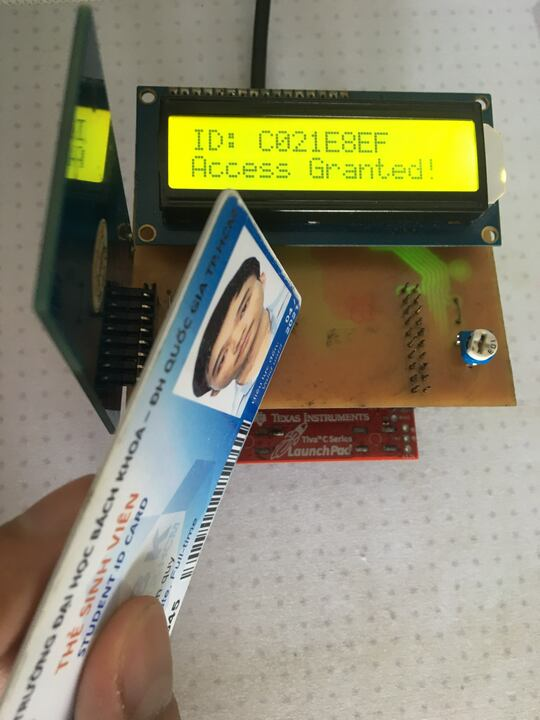
\includegraphics[scale=0.3]{images/mfrc522_student.jpg}
\caption{Kết quả hệ thống MFRC522 - Sử dụng thẻ sinh viên}
\label{fig:rc522_student}
\end{figure}

\clearpage
\subsection{Sử dụng một crate giải thuật cờ vua no-std trên kit Tiva C}
Một trong những điểm mạnh của Rust là các crate no-std có thể được sử dụng trên bất kỳ môi trường nào như đã giới thiệu ở phần trước.
Vì vậy, ở phần này, tôi thực hiện sử dụng một crate giải thuật cờ vua \mintinline{bash}{chess-engine} \cite{rust_chess_engine} mô phỏng một hệ thống đánh cờ vua blindfolded (không bàn cờ) đơn giản để chứng minh điều này.

Crate thực hiện giải thuật cờ vua này tương đối đơn giản, dựa trên hai giải thuật Minimax \cite{minimax_chess_programming} và Alpha-Beta Pruning \cite{alpha_beta_chess_programming}.
Người đọc có thể tham khảo về giải thuật này ở phần tài liệu tham khảo.

Trong phần này, tôi cũng sử dụng thêm một module bàn phím 4x4 để tăng tính tương tác với người dùng.
Nội dung của chương trình người đọc có thể tham khảo ở phần phụ lục. % TODO

Để thực hiện demo cho phần này, tôi thực hiện thiết lập một vị trí đơn giản như hình \ref{chess:start_fen}.
Ở đây, người chơi (điều khiển quân trắng) sẽ đi nước Qc6, cố tình tạo một thời cơ để cho máy tính (điều khiển quân đen) chơi một tactic 1. Bh2+ Kxh2 2. Qxc6.

\begin{figure}[ht]
\centering
\newchessgame
\def\fenstart{2kr2nr/p1p2ppp/1p1b2q1/3N4/2Q5/4B3/PPP2PPP/R3R1K1 w - - 4 16}
\chessboard[smallboard, setfen=\fenstart]

\mainline{1. Qc6??}
\caption{Ví trí ban đầu để thử nghiệm giải thuật cờ vua}
\label{chess:start_fen}
\end{figure}

\begin{figure}[ht]
\centering
\newchessgame
\def\fenbotezgambit{2kr2nr/p1p2ppp/1pQb2q1/3N4/8/4B3/PPP2PPP/R3R1K1 b - - 5 16}
\chessboard[smallboard, setfen=\fenbotezgambit]

\mainline{1. Bxh2+ Kxh2 2. Qxc6}
\caption{Ví trí sau khi đi nước Qc6 để máy tính bắt đầu tính toán}
\label{chess:botez_gambit}
\end{figure}

Một vài hình về kết quả thực hiện có thể xem ở các hình \ref{fig:chess_init}, \ref{fig:chess_c4c6}, \ref{fig:chess_wait_move2}, \ref{fig:chess_g1h2}, \ref{fig:chess_end}, \ref{fig:chess_illegal}.

\begin{figure}[ht]
\centering
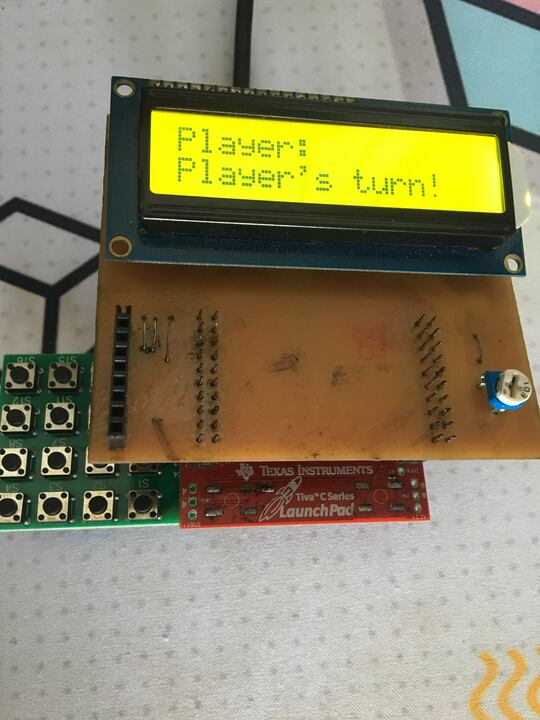
\includegraphics[scale=0.3]{images/chess_init.jpg}
\caption{Kết quả hệ thống MFRC522 - Hệ thống ở trạng thái mặc định như ở hình \ref{chess:start_fen}}
\label{fig:chess_init}
\end{figure}

\begin{figure}[ht]
\centering
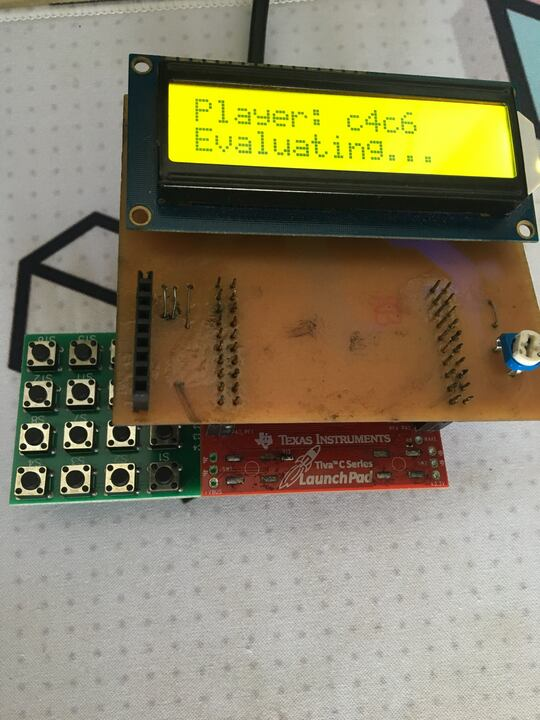
\includegraphics[scale=0.3]{images/chess_c4c6.jpg}
\caption{Kết quả hệ thống MFRC522 - Hệ thống đang giải nước Qc6}
\label{fig:chess_c4c6}
\end{figure}

\begin{figure}[ht]
\centering
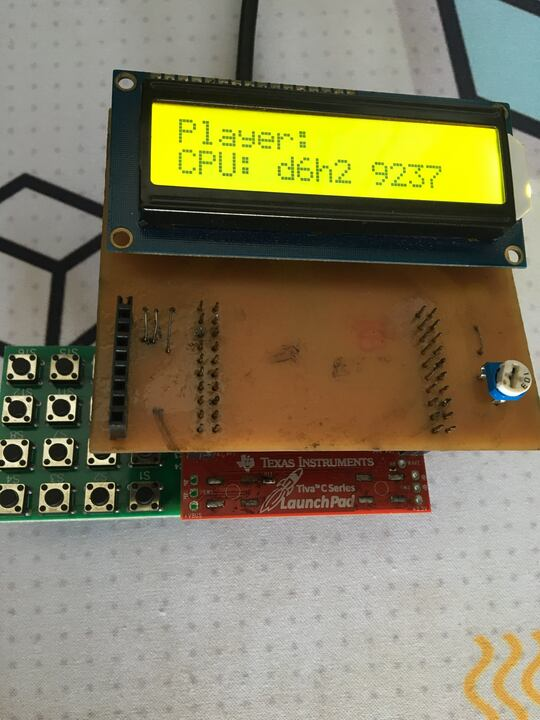
\includegraphics[scale=0.4]{images/chess_wait_move2.jpg}
\caption{Kết quả hệ thống MFRC522 - Hệ thống sau khi giải xong nước Qc6}
\label{fig:chess_wait_move2}
\end{figure}

\begin{figure}[ht]
\centering
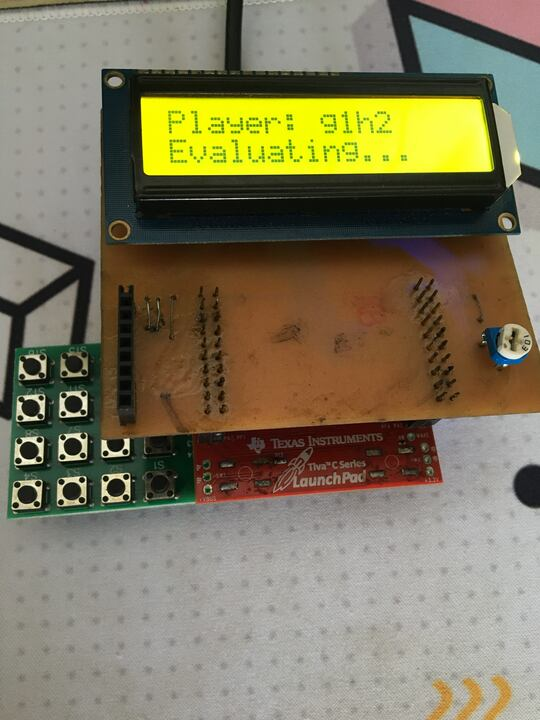
\includegraphics[scale=0.4]{images/chess_g1h2.jpg}
\caption{Kết quả hệ thống MFRC522 - Hệ thống đang giải nước Bxh2}
\label{fig:chess_g1h2}
\end{figure}

\begin{figure}[ht]
\centering
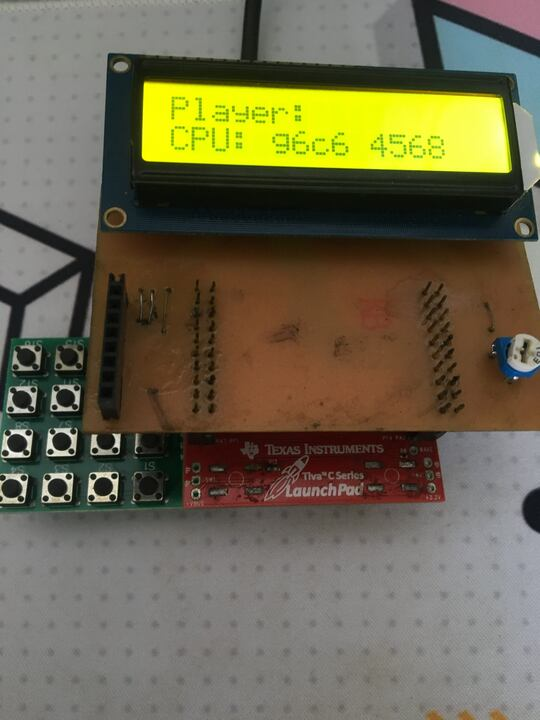
\includegraphics[scale=0.4]{images/chess_end.jpg}
\caption{Kết quả hệ thống MFRC522 - Hệ thống sau khi giải xong nước Bxh2}
\label{fig:chess_end}
\end{figure}

\begin{figure}[ht]
\centering
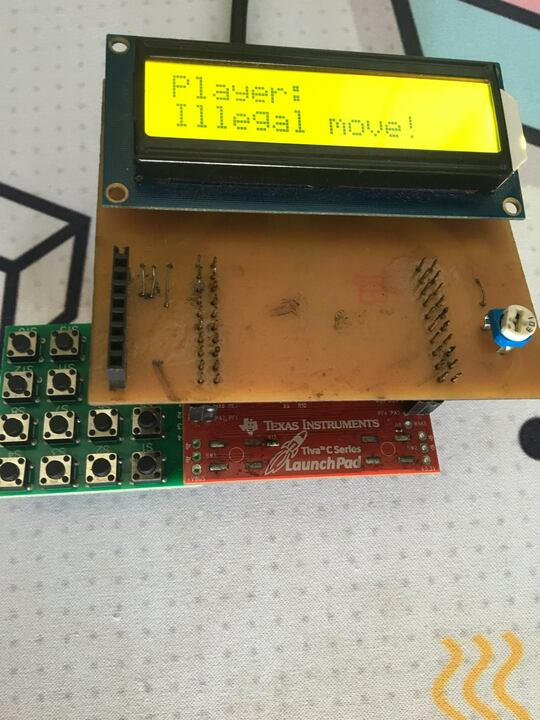
\includegraphics[scale=0.4]{images/chess_illegal.jpg}
\caption{Kết quả hệ thống giải thuật cờ vua - Người chơi đi nước không hợp lệ}
\label{fig:chess_illegal}
\end{figure}

\clearpage
\subsection{Sử dụng crate RTIC viết hệ thống real time sử dụng ngắt}
Một trong những cơ chế quan trọng trong việc viết những phần mềm nhúng nâng cao đó là sử dụng tính năng ngắt của vi điều khiển.
Trong phần này, tôi thực hiện sử dụng crate RTIC \cite{rtic_website} để viết một hệ thống nhúng real time sử dụng ngắt.

Hệ thống real time này là một hệ thống đơn giản, kết hợp các kiến thức đã thực hiện ở các phần \ref{lbl:rust_blinky} (trang \pageref{lbl:rust_blinky}), \ref{lbl:rust_peripheral} (trang \pageref{lbl:rust_peripheral}), \ref{lbl:rust_mfrc522} (trang \pageref{lbl:rust_mfrc522}) trước và kết hợp thêm một vài ví dụ nhỏ để mô tả chức năng scheduler của RTIC.

Hệ thống này gồm 5 tác vụ (tasks) trong đó 3 tác vụ là ngắt software và 2 tác vụ là ngắt hardware.
Hệ thống có các tính năng như sau:
\begin{itemize}
    \item Tác vụ LED: Nháy LED xanh dương sau mỗi 1s. Tương tự như phần \ref{lbl:rust_blinky} (trang \pageref{lbl:rust_blinky}), tuy nhiên ở đây sử dụng tính năng scheduler của RTIC.
    \item Tác vụ UART hardware: Thực hiện ngắt và đọc dữ liệu truyền đến kit qua UART. Tương tự hệ thống ở phần \ref{lbl:rust_peripheral} (trang \pageref{lbl:rust_peripheral}).
    \item Tác vụ LCD: Sau mỗi 0.5s tăng 1 vào một biến (ở đây là biến \mintinline{bash}{lcd_counter}) và xuất ra màn hình LCD.
    \item Tác vụ MFRC522: Thực hiện ngắt và đọc giá trị của thẻ RFID khi có thẻ được quét. Tương tự như hệ thống ở phần \ref{lbl:rust_mfrc522} (trang \pageref{lbl:rust_mfrc522}).
    \item Tác vụ UART software: Sau mỗi 2s xuất ra UART các giá trị của hệ thống như \mintinline{bash}{lcd_counter} và số thẻ đã đọc được ở tác vụ MFRC522 (biến \mintinline{bash}{card_counter}).
\end{itemize}

Nội dung của chương trình người đọc có thể tham khảo ở phần phụ lục. % TODO
Một vài hình về kết quả thực hiện có thể xem ở các hình \ref{fig:rtic_init}, \ref{fig:rtic_tag}, \ref{fig:rtic_card}, \ref{fig:rtic_student}, \ref{fig:rtic_uart}.

\begin{figure}[ht]
\centering
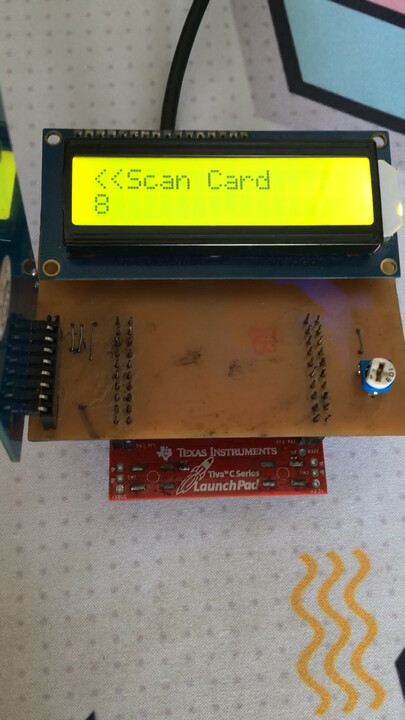
\includegraphics[scale=0.3]{images/rtic_init.jpg}
\caption{Kết quả hệ thống RTIC - Hệ thống ở trạng thái ban đầu}
\label{fig:rtic_init}
\end{figure}

\begin{figure}[ht]
\centering
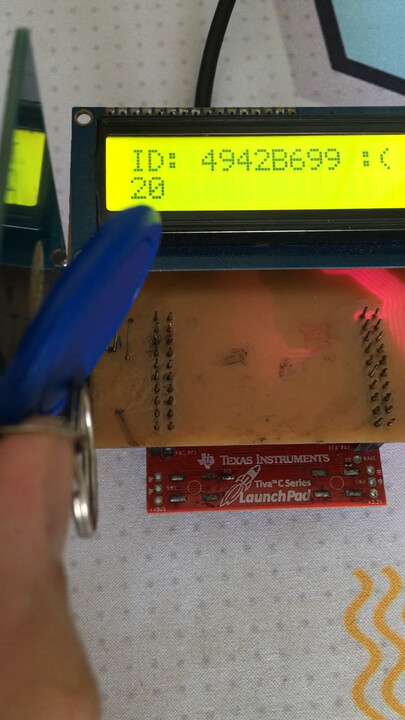
\includegraphics[scale=0.4]{images/rtic_tag.jpg}
\caption{Kết quả hệ thống RTIC - Hệ thống khi quét tag}
\label{fig:rtic_tag}
\end{figure}

\begin{figure}[ht]
\centering
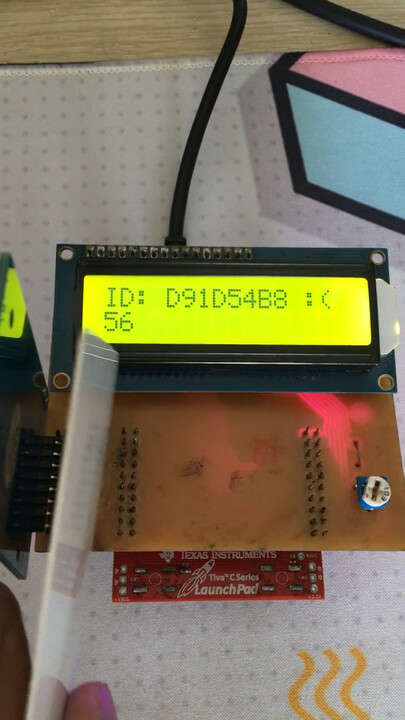
\includegraphics[scale=0.4]{images/rtic_card.jpg}
\caption{Kết quả hệ thống RTIC - Hệ thống khi khi quét card}
\label{fig:rtic_card}
\end{figure}

\begin{figure}[ht]
\centering
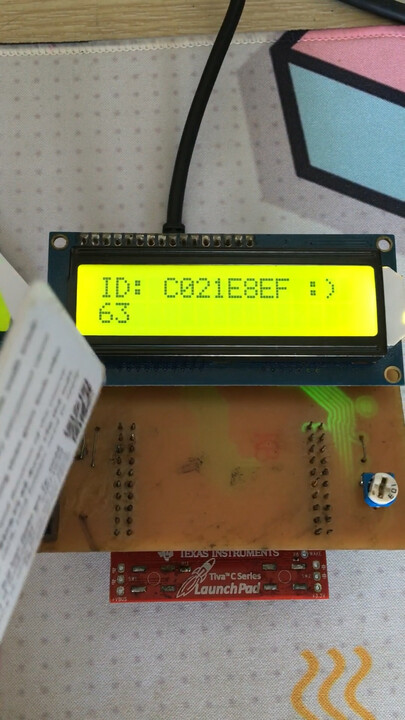
\includegraphics[scale=0.4]{images/rtic_student.jpg}
\caption{Kết quả hệ thống RTIC - Hệ thống khi quét thẻ sinh viên}
\label{fig:rtic_student}
\end{figure}

\begin{figure}[ht]
\centering
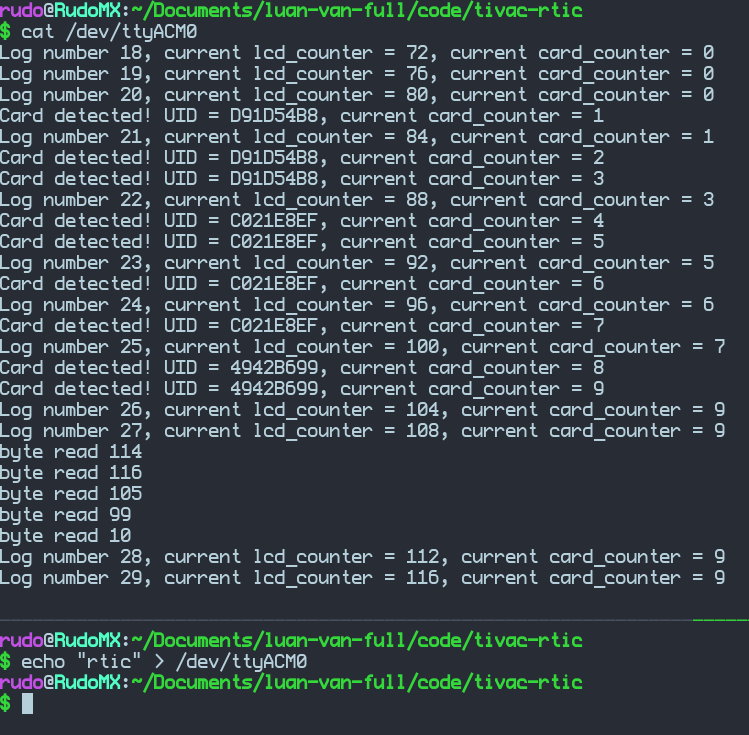
\includegraphics[scale=0.5]{images/rtic_uart.png}
\caption{Kết quả hệ thống RTIC - Hệ thống ghi và đọc cổng UART}
\label{fig:rtic_uart}
\end{figure}

\clearpage
Trong các phần thực hiện hệ thống thì phần sử dụng crate RTIC này, tôi gặp nhiều trục trặc về kỹ thuật nhất.
Các vấn đề trực trặc kỹ thuật này xuất phát từ cả hai crate đó là RTIC, cũng như là HAL chưa đầy đủ của kit Tiva C.
Một số khó khăn có thể được liệt kê ra như sau:
\begin{itemize}
    \item HAL của Tiva C ở thời điểm viết bài chưa hỗ trợ ngắt trực tiếp UART cũng như SSI.
        Hiện tại hệ thống sử dụng ngắt GPIO để thay thế, vì vậy bị mất đi các chân GPIO sử dụng để ngắt khi thực hiện điều này.
    \item HAL của Tiva C hiện tại chỉ có một cách tạo biến delay duy nhất đó là sử dụng SysTick, tuy nhiên RTIC lại sử dụng SysTick cho monotonic scheduler.
        Vì vậy người dùng monotonic scheduler phải thực hiện viết cách tạo delay khác.
        Ở đây tôi chọn cách sử dụng countdown timer trên kit để tạo delay.
    \item RTIC sử dụng các phương pháp quản lý tài nguyên hệ thống cũng như switch task tương đối khác so với hệ thống RTOS quen thuộc nên đã gây một số hiểu lầm trong quá trình thực hiện hệ thống.
\end{itemize}

Tuy nhiên về cơ bản thì việc thực hiện hệ thống sử dụng crate RTIC là tương đối đơn giản và dễ dàng.
Crate RTIC kết hợp chặt chẽ với hệ thống ownership của Rust ngăn chặn được nhiều lỗi trong hệ thống ngắt nói chung như datarace thông qua hệ thống resource lock của mình.
